\section{Multi-Layer Perceptron Classifier}
	    \pagestyle{mario}
	    \sectionauthor{M. Gini \& T. M. Hayden} %\printinunitsof{cm}\prntlen{\linewidth} this shows linewidth in cm

This section presents the multi-layer perceptron (MLP) classifier designed to classify the CIFAR-10 dataset. It is organized as follows: Section \ref{subsec:setup} introduces the software setup used to implement the MLP classifier. Section \ref{subsec:preProp} discusses the data preprocessing and augmentation. Section \ref{subsec:netStruct} analyzes the effect of different network structures on performance. Section \ref{subsec:optNet} analyzes the effect of different hyperparameters.

\subsection{Software Setup}\label{subsec:setup}

MATLAB's Neural Networks toolbox is employed to implement the MLP classifier. The toolbox provides convenient algorithms and applications to design the MLP. A network training function with a convenient graphical user interface (GUI) to observe the progress is included as well. Figure \ref{fig:NNtool} shows the GUI.

Since this is a classification problem, parts of the network structure are given. The output of the MLP should be a prediction of to which class the input belongs to. This is accomplished with the help of the softmax function, also called normalized exponential function. Equation \ref{eq:softmax} shows the formula of such a function. A softmax layer is then used as the last layer. It gets a $K$-dimensional input vector $\boldsymbol{z}$ of arbitrary real values and "squashes" it into a $K$-dimensional output vector $\sigma(\boldsymbol{z})$ of real values in the range $[0,1]$. In our case, $K=10$ and the output values represent the probabilities that the input belongs to the respective class. The class with the highest probability then constitutes the predicition of the MLP.

\begin{equation}\label{eq:softmax}
\sigma(\boldsymbol{z})_j = \frac{e^{z_j}}{\sum_{k=1}^{K}e^{z_k}}\quad \textrm{for}\quad j = 1,...~K.
\end{equation}

\begin{figure}[h!]
  	\centering
  	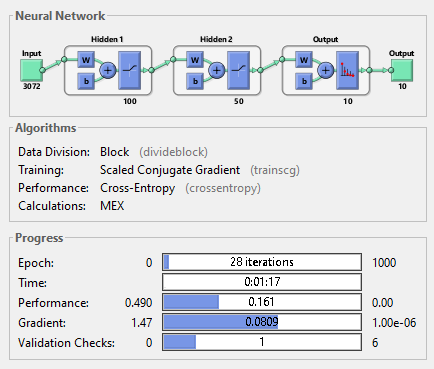
\includegraphics{images/NNtool}
  	\caption{Screenshot of MATLAB's nntraintool.}
  	\label{fig:NNtool}
\end{figure}

The other hidden layers consist of standard MLP. MATLAB offers lots of adjustable settings for the MLP. Unless mentioned otherwise, the following settings are employed as default settings:

\begin{itemize}
	\item Training function: 
	
	\item Loss function: cross entropy
	
	\item Activation function: 'tansig', the hyperbolic tangent sigmoid activation function 
	
	\item Training batch size: 20000 images
	
	\item Network structure: Two hidden layers, 100 neurons on the first layer and 50 neurons on the second layer.
\end{itemize}

a) on the selection of the inputs and outputs of the MLP

\FloatBarrier
\subsection{Data Preprocessing and Augmentation}\label{subsec:preProp}
Data preprocessing and augmentation.

b) on the size of the training data 
 
\subsubsection{Data Preprocessing}\label{subsub:dataPreProp}

  	The input data is to the network consists of a 3072*1 array where the entries represent the raw pixel values. The pixel values are in the range [0,255]. To avoid any numerical issues and normalize the data, the data is divided by 255 to lie within the range [0,1]. Accordingly, the datatype is changed from the integer format to double. In a second step, the mean per pixel over the whole training set is subtracted. This centers the data.
  	
  	Optionally, we conduct experiments with whitened data. \textcolor{red}{here some plot to show effect of whitened data}
  	  	
  	\begin{figure}[h!]
  		\centering	  		
  		\includegraphics{images/numberlayers}
  	  	\caption{Hello Boy2}
  	  	\label{fig:test2}
  	 \end{figure}
  	
  	Data preprocessing also includes the division of the complete dataset into appropriate training, validation and test data batches. The CIFAR-10 dataset consists of 60000 images, with 10000 specifically labeled for testing. For our performance analysis, we always use the provided test batch. The effect of varying training batch size can be seen below \textcolor{red}{here some plot of varying training size}
  	
\subsubsection{Data Augmentation}
	    	
   	Experience shows that a larger training data set increases network performance. A basic and still successful data augmentation method is vertical mirroring. \textcolor{red}{here some plot of varying training size with mirrored data} When comparing with above, the increase in performance can clearly be seen.
   	
   	\begin{figure}[h!]
		\centering
   	  	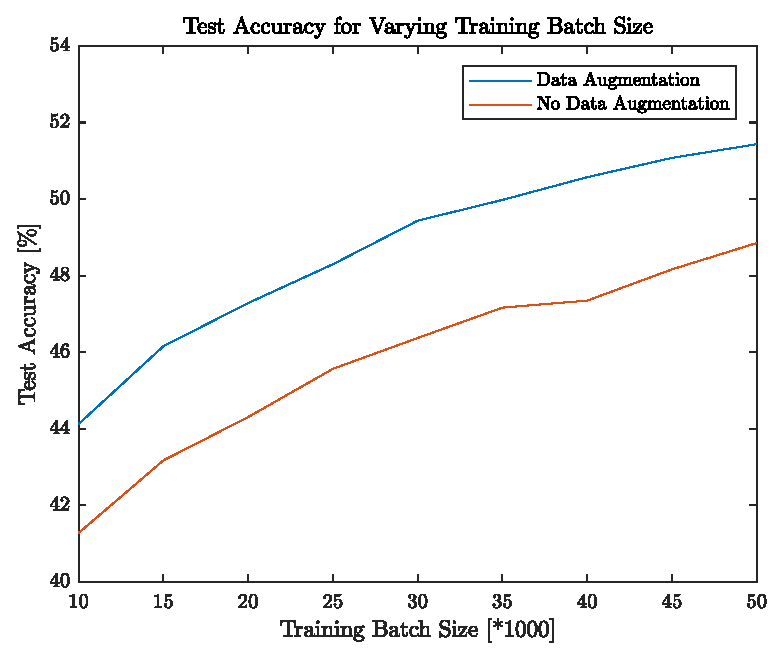
\includegraphics{images/dataAugmentation}
   	  	\caption{Hello Boy}
   	  	\label{fig:test1}
   	\end{figure}
   		    
\subsection{Optimization of Network Structure}\label{subsec:netStruct}
c)on the training of the MLP    
\begin{itemize}
   	\item Varying the number of neurons	
	\item Varying the number of layers	    	
\end{itemize}
	    
\subsection{Optimization of Network Hyperparameters}\label{subsec:optNet}
d) on the performance of the MLP with different objective functions and optimization methods

\textcolor{red}{Some pic of the confusion matrix}

\begin{itemize}
   	\item Different learning rates
	    	
   	\item Different optimization methods
\end{itemize}
e)any other interesting observation that you think are pertinent (e.g. effect of learning rate on convergence speed).